
\subsection*{Hints for Review Question~\ref{ge5}}

%%%Insert this to get the typewriter font so it looks like a real movie script
{\ttfamily
\fontdimen2\font=0.4em
\fontdimen3\font=0.2em
\fontdimen4\font=0.1em
\fontdimen7\font=0.1em
\hyphenchar\font=`\-


%%%%put a hypertarget around the opening bit of text
%\hypertarget{script_gaussian_elimination_hints}{The hint} for Review Question~\ref{ge4} is simple--just read the lecture on 
%\hyperlink{Elementary Row Operations}{Elementary Row Operations}. 

\hypertarget{script_gaussian_elimination_hints}{This} question looks harder than it actually is:

\begin{quote}{\small
Row equivalence of matrices is an example of an \emph{equivalence relation}.  Recall that a relation $\sim$ on a set of objects $U$ is an equivalence relation if the following three properties are satisfied:
\begin{itemize}
\item Reflexive:  For any $x\in U$, we have $x\sim x$.
\item Symmetric:  For any $x,y \in U$, if $x\sim y$ then $y\sim x$.
\item Transitive: For any $x,y$ and $z \in U$, if $x\sim y$ and $y\sim z$ then $x\sim z$.
\end{itemize}

(For a more complete discussion of equivalence relations, see \href{\webworkurl Homework0-Background/4/}{Webwork Homework 0, Problem 4})

Show that row equivalence of augmented matrices is an equivalence relation.
}
\end{quote}

Firstly remember that an equivalence relation is just a more general version of ``equals''.
Here we defined row equivalence  for augmented matrices whose linear systems have
solutions by the property that their solutions are the same.

So this question is really about the word {\it same}. Lets do a silly example:
Lets replace the set of augmented matrices by the set of people who have hair.
We will call two people equivalent if they have the same hair color. There are three properties
to check:

\begin{itemize}
\item Reflexive: This just requires that you have the same hair color as yourself so obviously holds.

\begin{center}
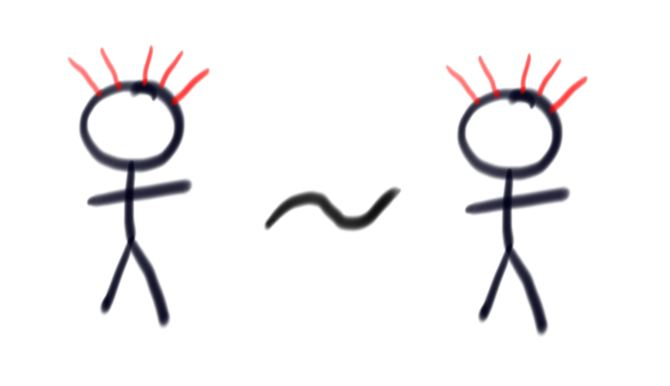
\includegraphics[scale=.15]{bobbob.jpg}
\end{center}

\item Symmetric: If the first person, Bob (say) has the same hair color as a second person Betty(say), then Bob has
the same hair color as Betty, so this holds too.

\begin{center}
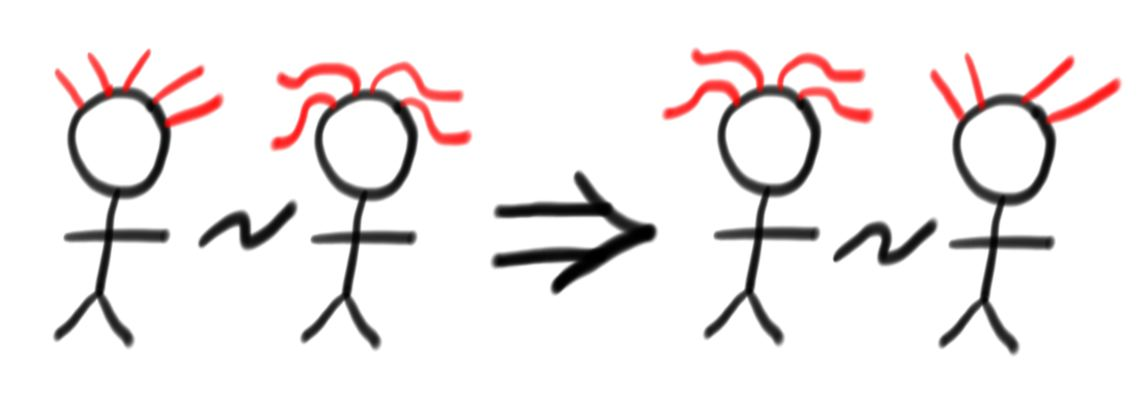
\includegraphics[scale=.15]{bobbetty.jpg}
\end{center}

\item Transitive: If Bob has the same hair color as Betty (say) and Betty has the same color as Brenda (say), then it follows
that Bob and Brenda have the same hair color, so the transitive property holds too and we are done.

\begin{center}
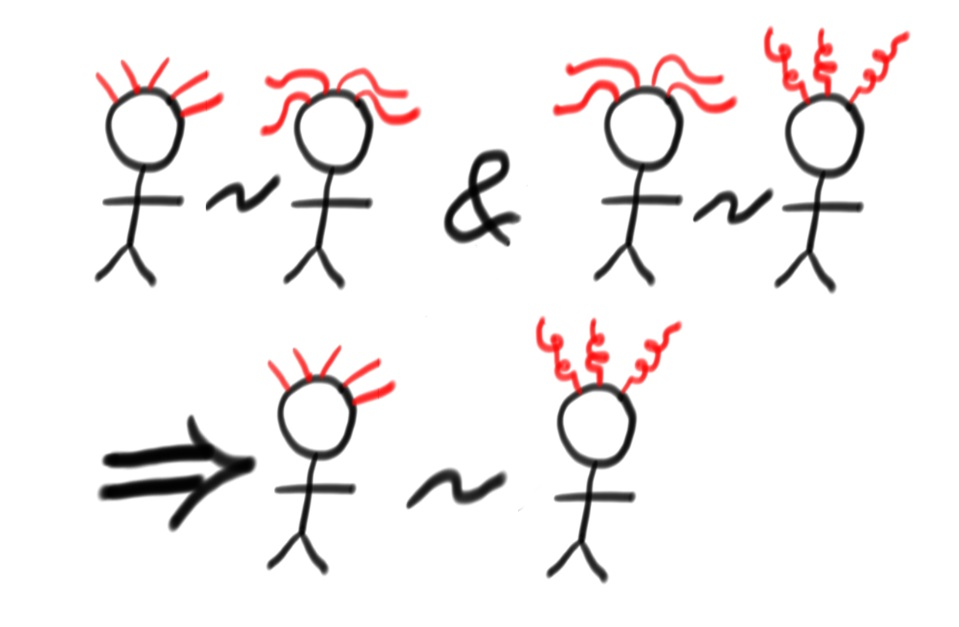
\includegraphics[scale=.24]{bobbettybrenda.jpg}
\end{center}
\end{itemize}
%%%%don't forget to close the bracket so the stuff after your file doesn't look like a movie!
}

\newpage
